% Compile with XeLaTeX. Protocol 1 original text + Protocol 2 review notes.

% Source: supplied photographs, pp. 156--160, section 7.1.1 only.

% This is a separate document based on the supplied formatting example.

\documentclass[11pt,a4paper,twoside]{article}

\usepackage{fontspec}

\usepackage{xeCJK}

\IfFontExistsTF{Times New Roman}{\setmainfont{Times New Roman}}{\setmainfont{Latin Modern Roman}}

\ifdefined\setCJKmainfont

\IfFontExistsTF{Noto Serif TC}{\setCJKmainfont{Noto Serif TC}}{\setCJKmainfont{FandolSong-Regular}}

\fi

\usepackage{amsmath,amssymb,mathtools,empheq}

\usepackage[most]{tcolorbox}

\usepackage{tikz,wrapfig}

\usepackage[a4paper,inner=2.5cm,outer=2cm,top=2.5cm,bottom=2.5cm]{geometry}

\usepackage{setspace}

\setstretch{1.25}

\setlength{\parindent}{2em}

\setlength{\parskip}{5pt}

\setlength{\abovedisplayskip}{6pt}

\setlength{\belowdisplayskip}{6pt}

\setlength{\abovedisplayshortskip}{4pt}

\setlength{\belowdisplayshortskip}{4pt}

\usepackage{fancyhdr}

\usepackage[hang,flushmargin]{footmisc}

\pagestyle{fancy}

\fancyhf{}

\renewcommand{\headrulewidth}{0pt}

\fancyfoot[RO,LE]{\small $\boldsymbol{\cdot}\;\thepage\;\boldsymbol{\cdot}$}

\newcommand{\pnum}[1]{\makebox[0pt][r]{\scriptsize\textbf{[#1]}\hspace{0.7em}}}

\newif\ifstudynotes

\studynotestrue

\newtcolorbox{studyNote}[1][]{enhanced,breakable,colback=gray!4,colframe=black!35,boxrule=0.5pt,arc=1mm,left=2mm,right=2mm,top=1.5mm,bottom=1.5mm,before skip=6pt,after skip=8pt,fonttitle=\bfseries,title={複習註解},#1}

\newtcolorbox{importantNote}[1][]{enhanced,breakable,colback=gray!8,colframe=black!65,boxrule=0.8pt,arc=1mm,left=2mm,right=2mm,top=1.5mm,bottom=1.5mm,before skip=7pt,after skip=9pt,fonttitle=\bfseries,title={重要觀念},#1}

\newcommand{\StudyNote}[2]{\ifstudynotes\begin{studyNote}[title={#1}]#2\end{studyNote}\fi}

\newcommand{\ImportantNote}[2]{\ifstudynotes\begin{importantNote}[title={#1}]#2\end{importantNote}\fi}

\begin{document}

\setcounter{page}{156}

% Original page 156: only the requested section is included.

\noindent{\large\bfseries 7.1.1\quad The Euler--Lagrange Equations}

\par\vspace{0.6em}\hrule\vspace{0.8em}

\noindent\pnum{1}Given some functional $F[y(x)]\in\mathbb{R}$, it's natural to ask: For which functions $y(x)$ does $F[y(x)]$ take its maximum value? And for which does it take its minimum value?



% --- Original page 157 ---

\noindent\pnum{2}The answer to these questions comes from taking some trial function $y(x)$ and then varying it to some nearby path $y(x)+\delta y(x)$ to see if the functional $F[y(x)]$ increases or decreases in value. This is where the name ``calculus of variations'' comes from.



\noindent\pnum{3}To see how this works in practice, let's first remind ourselves of the situation when we have a function $f(y_1,\ldots,y_n)$ of several variables. We consider the value of the function at some point $\mathbf{y}=(y_1,\ldots,y_n)$ and then compare to a neighbouring point $\mathbf{y}+\delta\mathbf{y}$. If we Taylor expand, we have

\begin{equation}
    f(\mathbf{y}+\delta\mathbf{y})=f(\mathbf{y})+\frac{\partial f}{\partial y_i}(\mathbf{y})\,\delta y_i+\frac12\frac{\partial^2 f}{\partial y_i\partial y_j}(\mathbf{y})\,\delta y_i\delta y_j+\cdots .\tag{7.5}
\end{equation}

\noindent\pnum{4}We say that the original point $\mathbf{y}$ is a \textit{stationary point} if the function does not change to leading order in $\delta\mathbf{y}$, so that

\begin{equation}
    \frac{\partial f}{\partial y_i}(\mathbf{y})=0\quad\text{for all }i=1,\ldots,n.\tag{7.6}
\end{equation}

\noindent\pnum{5}We've not yet determined whether this stationary point is a maximum or a minimum or something else. For that, we need to look at the second-order term in the expansion. We'll postpone this to Section 7.1.3.



\noindent\pnum{6}Now we repeat this story for functionals rather than functions. Consider a functional $F[y(x)]$ given by the general form

\begin{equation}
    F[y(x)]=\int_a^b dx\ L\bigl(y(x),y'(x),x\bigr).\tag{7.7}
\end{equation}

\noindent\pnum{7}We evaluate this on two nearby functions, $y(x)$ and $y(x)+\delta y(x)$. We're interested in the difference between them

\begin{equation}
    \delta F[y]=F[y+\delta y]-F[y].\tag{7.8}
\end{equation}

\noindent\pnum{8}Working to leading order in $\delta y(x)$, we have

\begin{equation}
    \begin{aligned}
        \delta F[y] & =\int_a^b dx\ L(y+\delta y,y'+\delta y',x)-\int_a^b dx\ L(y,y',x)                                               \\
                    & =\int_a^b dx\left[\frac{\partial L}{\partial y}\delta y+\frac{\partial L}{\partial y'}\delta y'\right]+\cdots .
    \end{aligned}\tag{7.9}
\end{equation}



% BEGIN PROTOCOL 2 NOTE: Taylor expansion

\StudyNote{複習註解：由 (7.7) 到 (7.9)}{

    把 $y(x)$ 改成 $y(x)+\delta y(x)$ 時，導數同時改成

    \[
        (y+\delta y)'=y'+\delta y',\qquad
        \delta y'=\frac{d}{dx}(\delta y).
    \]

    因此 $F[y+\delta y]$ 的被積函數是 $L(y+\delta y,y'+\delta y',x)$。

    在同一個固定的 $x$，依 (7.5) 對 $L$ 的前兩個引數做泰勒展開：

    \[
        L(y+\delta y,y'+\delta y',x)
        =L(y,y',x)+\frac{\partial L}{\partial y}\delta y
        +\frac{\partial L}{\partial y'}\delta y'+\cdots .
    \]

    偏導數都在原本的 $(y(x),y'(x),x)$ 處取值；$x$ 沒有變動，故沒有

    $(\partial L/\partial x)\delta x$ 項。減去原本的 $L$ 再積分，即得 (7.9)。

    省略的是 $(\delta y)^2$、$\delta y\,\delta y'$、$(\delta y')^2$ 等二階以上的項。



    例如 $L=y^2+(y')^2$，直接相減可得

    \[
        \Delta L=2y\,\delta y+2y'\,\delta y'+(\delta y)^2+(\delta y')^2.
    \]

    保留一階項，正好就是 $L_y\delta y+L_{y'}\delta y'$。

}

% END PROTOCOL 2 NOTE



\noindent\pnum{9}Here the $\ldots$ are terms that we've neglected of order $\delta y^2$. We see that, to leading order, $\delta F[y]$ depends on two terms, one proportional to $\delta y$ and the other to $\delta y'$. We can put these on the same footing by integrating the second term by parts

\begin{equation}
    \delta F[y]=\int_a^b dx\left[\frac{\partial L}{\partial y}-\frac{d}{dx}\left(\frac{\partial L}{\partial y'}\right)\right]\delta y(x)+\left[\frac{\partial L}{\partial y'}\delta y\right]_a^b.\tag{7.10}
\end{equation}



% BEGIN PROTOCOL 2 NOTE: Integration by parts

\StudyNote{複習註解：由 (7.9) 到 (7.10)}{

    這一步使用分部積分。因為 $\delta y'=d(\delta y)/dx$，令

    \[
        u=\frac{\partial L}{\partial y'},\qquad dv=\delta y'\,dx,
        \qquad v=\delta y.
    \]

    套用 $\int u\,dv=[uv]_a^b-\int v\,du$，得到

    \[
        \int_a^b\frac{\partial L}{\partial y'}\delta y'\,dx
        =\left[\frac{\partial L}{\partial y'}\delta y\right]_a^b
        -\int_a^b\frac{d}{dx}\left(\frac{\partial L}{\partial y'}\right)\delta y\,dx.
    \]

    代回 (7.9)，把兩個含 $\delta y$ 的積分合併，就得到 (7.10)。

    這裡的 $d/dx$ 是全導數：$\partial L/\partial y'$ 仍可能透過

    $y(x)$、$y'(x)$ 或顯含的 $x$ 隨 $x$ 改變。

    若兩端點固定，$\delta y(a)=\delta y(b)=0$，邊界項便消失。

}

% END PROTOCOL 2 NOTE





% --- Original page 158 ---

\noindent\pnum{10}We will ask that the boundary term vanishes. We can achieve this in one of two ways:

\begin{itemize}

    \item \pnum{11}We could fix the value of $y(x)$ at $x=a$ and $x=b$. This means that we only evaluate the functional $F[y(x)]$ on the curves with certain specified boundary conditions, $y(a)$ and $y(b)$, which ensures that, when varying the curves, we must have $\delta y(a)=\delta y(b)=0$.

    \item \pnum{12}Alternatively, we could require that $\partial L/\partial y'=0$ at $x=a$ and $x=b$. For many purposes, $L(y,y',x)$ is quadratic or higher in $y'$, in which case we can ensure this boundary condition by requiring $y'(a)=y'(b)=0$. These are usually referred to as \textit{free boundary conditions}.

    \item \pnum{13}We could have a mixed boundary condition, fixed at one end and free at the other.

\end{itemize}

\noindent\pnum{14}If the boundary term vanishes, then the variation of the functional $F[y(x)]$ is given by the first integral term in (7.10). We will say that the initial function $y(x)$ is a \textit{stationary point} or \textit{extremum} of $F[y(x)]$ if $\delta F[y(x)]=0$ for all variations $\delta y(x)$ that satisfy the required boundary condition. (The term ``stationary point'' is slightly misleading here because the ``point'' in question is now an entire function $y(x)$.)



\noindent\pnum{15}The fact that $\delta F[y(x)]$ must vanish for all variations $\delta y(x)$ is important. The only way that this can happen is if the term in square brackets in the integrand of (7.10) itself vanishes, meaning

\begin{equation}
    \frac{\partial L}{\partial y}-\frac{d}{dx}\left(\frac{\partial L}{\partial y'}\right)=0.\tag{7.11}
\end{equation}



% BEGIN PROTOCOL 2 NOTE: Purpose of integration by parts

\StudyNote{複習註解：維持 (7.9) 不好嗎？}{

    \textbf{(7.9) 本身正確。}分部積分是為了從駐定條件讀出 $y$ 滿足的微分方程式。

    因為 $\delta y'=d(\delta y)/dx$，選定 $\delta y$ 後，$\delta y'$ 就跟著確定；

    不能把兩者當成可獨立選擇的變動，分別要求 $L_y=0$ 與 $L_{y'}=0$。



    分部積分並消去邊界項後，一階變化成為

    \[
        \delta F=\int_a^b G(x)\,\delta y(x)\,dx,
        \qquad G(x)=\frac{\partial L}{\partial y}
        -\frac{d}{dx}\left(\frac{\partial L}{\partial y'}\right).
    \]

    駐定要求它對\textbf{所有容許的變動}皆為零。若連續的 $G$ 在某處為正，

    可在附近選取一個非負、光滑且只在該小區域內非零的 $\delta y$，使積分大於零；

    為負時同理。因此必須 $G(x)=0$，這就是 (7.11)。



    \textbf{檢查例子：}若 $L=\tfrac12(y')^2$，固定端點下

    \[
        \delta F=\int_a^b y'\delta y'\,dx
            =[y'\delta y]_a^b-\int_a^b y''\delta y\,dx
        =-\int_a^b y''\delta y\,dx.
    \]

    正確條件是 $y''=0$，所以 $y=mx+c$。

    若誤把 (7.9) 中 $\delta y'$ 的係數直接設零，就會得到過強的條件 $y'=0$，排除斜直線。

}

% END PROTOCOL 2 NOTE



\noindent\pnum{16}This is the \textit{Euler--Lagrange equation}. Functions $y(x)$ that obey this equation are extrema of the functional $F[y(x)]$.



\newpage

\begin{center}\large\bfseries An Example: Geodesics on a Plane\end{center}

\noindent\pnum{17}Here's a simple, and trivial, application of this result. We will determine the shortest path that connects two points on a plane, say $(x,y)=(a,A)$ and $(x,y)=(b,B)$. The name given to a shortest path on some space is a \textit{geodesic}.



\noindent\pnum{18}The length of a curve $y(x)$ in the plane is given by the functional (7.3)

\begin{equation}
    F[y(x)]=\int_a^b dx\ \sqrt{1+y'(x)^2}.\tag{7.12}
\end{equation}

\noindent\pnum{19}In this case, we minimise over all curves with fixed end points, which means

% --- Original page 159: continuation of paragraph [19]. ---

\noindent that we have the boundary conditions $\delta y(a)=\delta y(b)=0$. The integrand of the functional $L=\sqrt{1+y'^2}$ depends only on $y'$ and so $\partial L/\partial y=0$ and the Euler--Lagrange equation reads

\begin{equation}
    \frac{d}{dx}\left(\frac{\partial L}{\partial y'}\right)=\frac{d}{dx}\left(\frac{y'}{\sqrt{1+y'^2}}\right)=0.\tag{7.13}
\end{equation}

\noindent\pnum{20}This is solved by curves $y(x)$ such that $y'(x)=\text{constant}$. Imposing the boundary conditions $y(a)=A$ and $y(b)=B$, we have the unique solution

\begin{equation}
    y=\alpha x+\beta\quad\text{with}\quad\alpha=\frac{B-A}{b-a}\quad\text{and}\quad\beta=\frac{bA-Ba}{b-a}.\tag{7.14}
\end{equation}

\noindent\pnum{21}We learn that the shortest path between two points on the plane is a straight line. That, of course, is deeply unsurprising.



\newpage

\begin{center}\large\bfseries Another Example: Geodesics on a Sphere\end{center}

\noindent\pnum{22}As another example, we can determine the shortest distance between two points on a sphere. This time the story is a little more intricate. The first thing that we need to do is to write down the functional that describes the length of a general curve on a sphere.



\noindent\pnum{23}We embed our sphere in $\mathbb{R}^3$ with the usual spherical polar coordinates

\begin{equation}
    x=R\sin\theta\cos\phi,\quad y=R\sin\theta\sin\phi,\quad z=R\cos\theta.\tag{7.15}
\end{equation}

\noindent\pnum{24}Consider two nearby points on the sphere, $(\theta,\phi)$ and $(\theta+\delta\theta,\phi+\delta\phi)$. What is the distance $\delta s$ between these two points? We can determine this by substituting the polar decomposition above into the usual Pythagorean distance $\delta s^2=\delta x^2+\delta y^2+\delta z^2$, keeping the radius $R$ fixed. We have

\begin{equation}
    \delta s^2=\delta\theta^2+\sin^2\theta\,\delta\phi^2.\tag{7.16}
\end{equation}

\noindent\pnum{25}At this point, there are various ways to proceed. We could, for example, think of a path on the sphere as given by $\phi=\phi(\theta)$. Then the analog of our flat-plane functional (7.12) for the length of the path is

\begin{equation}
    F[\phi(\theta)]=\int_{\theta_1}^{\theta_2}d\theta\ \sqrt{1+\sin^2\theta\,\phi'(\theta)^2}.\tag{7.17}
\end{equation}

\noindent\pnum{26}We could then proceed to solve the corresponding Euler--Lagrange equation. However, it turns out to be a little cumbersome and there's a slicker way forward. To this end, instead of thinking of $\phi=\phi(\theta)$, we will instead consider a path on the sphere to be given by $\theta(t)$ and $\phi(t)$, where $t$ is some parameter

% --- Original page 160: continuation of paragraph [26]. ---

\noindent along the path. The length of such a parameterised path is given by

\begin{equation}
    F[\theta(t),\phi(t)]=\int_{t_1}^{t_2}dt\ \sqrt{\dot\theta^2+\sin^2\theta\,\dot\phi^2}\tag{7.18}
\end{equation}

% BEGIN PROTOCOL 2 NOTE: Parameterised arc length
\StudyNote{複習註解：式 (7.18) 的參數化弧長}{
    改用參數 $t$ 描述路徑，令 $\theta=\theta(t)$、$\phi=\phi(t)$，則
    \[
        d\theta=\dot\theta\,dt,\qquad d\phi=\dot\phi\,dt.
    \]
    將它們代入單位球的弧長公式 (7.16)：
    \[
        \begin{aligned}
            ds^2 & =(d\theta)^2+\sin^2\theta\,(d\phi)^2                       \\
                 & =\left(\dot\theta^2+\sin^2\theta\,\dot\phi^2\right)(dt)^2.
        \end{aligned}
    \]
    讓 $t$ 沿路遞增，取平方根並積分：
    \[
        F[\theta(t),\phi(t)]=\int_{t_1}^{t_2}
        \sqrt{\dot\theta^2+\sin^2\theta\,\dot\phi^2}\,dt.
    \]
    這就是 (7.18)。$t$ 只是路徑參數，不一定是時間；點號表示對 $t$ 微分。

    \textbf{與 (7.17) 的關係：}若選擇 $t=\theta$，則
    \[
        \dot\theta=1,\qquad \dot\phi=\phi'(\theta),
    \]
    (7.18) 就回到 (7.17)。因此，原先根號內的 $1$，在一般參數下變成了 $\dot\theta^2$。
    若球半徑為一般的 $R$，上述弧長與總長度須再乘上 $R$。
}
% END PROTOCOL 2 NOTE


% Vector reconstruction of the unnumbered source figure.

\begin{wrapfigure}{r}{0.37\textwidth}

    \centering

    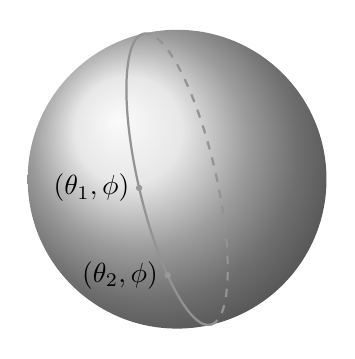
\begin{tikzpicture}[scale=1.15]

        \shade[ball color=gray!25] (0,0) circle (1.65);

        \begin{scope}[rotate=13]

            \draw[gray!85,thick] (0,1.65) arc[start angle=90,end angle=270,x radius=.43,y radius=1.65];

            \draw[gray!85,thick,dashed] (0,-1.65) arc[start angle=270,end angle=450,x radius=.43,y radius=1.65];

            \fill[gray!80] (-.43,0) circle (.035) node[left,black] {$(\theta_1,\phi)$};

            \fill[gray!80] (-.34,-1.01) circle (.035) node[left,black] {$(\theta_2,\phi)$};

        \end{scope}

    \end{tikzpicture}

\end{wrapfigure}

\noindent with $\dot\theta=d\theta/dt$ and $\dot\phi=d\phi/dt$. This is a generalisation of what we had previously: now it is a functional of two functions $\theta(t)$ and $\phi(t)$, rather than just one. Correspondingly, there are two Euler--Lagrange equations, one for each function. However, there's a more direct way to minimise this functional that doesn't require us to derive the Euler--Lagrange equations. For this, we first use the rotational symmetry of the sphere to align our polar coordinates so that both the start and end points of the curve have the same $\phi$ value, as shown on the figure. This $\phi=\text{constant}$ curve is a great circle. We then note the following chain of inequalities

\begin{equation}
    F[\theta(t),\phi(t)]\geq\int_{t_1}^{t_2}dt\ |\dot\theta|\geq|\theta_2-\theta_1|\tag{7.19}
\end{equation}

\noindent\pnum{27}The first inequality is saturated whenever $\dot\phi=0$, so that the path is along the great circle that joins the two points. The second inequality is saturated whenever $\theta(t)$ is monotonic, so that the path doesn't double back on itself. When both of these conditions are met, the inequalities are equalities and the distance along the path is $F=|\theta_2-\theta_1|$. We learn that the geodesics that minimise the functional $F[\theta(t),\phi(t)]$ are great circles between the two points. Note that this argument doesn't tell us which direction around the sphere we should go. In one direction, the geodesic is a global minimum of $F$; in the other direction, going the long way around the back of the sphere, the geodesic is a local minimum.


% BEGIN PROTOCOL 2 NOTE: Equality conditions in paragraph 27
\StudyNote{複習註解：式 (7.19) 何時取等號？}{
    原文的 ``the inequality is saturated'' 是指「不等式取等號」。

    \textbf{第一個不等式：}
    \[
        F=\int_{t_1}^{t_2}
        \sqrt{\dot\theta^2+\sin^2\theta\,\dot\phi^2}\,dt
        \geq\int_{t_1}^{t_2}|\dot\theta|\,dt.
    \]
    若 $\dot\phi=0$，即 $\phi$ 保持常數，多出的非負項消失，便取等號。
    幾何上，就是沿著前面選好的子午線走。

    \textbf{第二個不等式：}
    \[
        \int_{t_1}^{t_2}|\dot\theta|\,dt
        \geq\left|\int_{t_1}^{t_2}\dot\theta\,dt\right|
        =|\theta_2-\theta_1|.
    \]
    左邊是 $\theta$ 的總變化量，右邊是淨變化量的大小。
    若 $\theta(t)$ 單調、不折返（允許暫停），就取等號。

    因此，在前面選定的座標下，沿連接兩端點的短大圓弧行走，
    保持 $\phi$ 不變且 $\theta$ 單調，就能同時達到兩個等號：
    \[
        \boxed{F=|\theta_2-\theta_1|.}
    \]
    這條路徑達到長度下界，所以最短。若球半徑為 $R$，長度須再乘上 $R$。

    \textbf{原文末句辨正：}對非對跖的兩端點，繞另一邊、超過半圈的長大圓弧，
    雖然也是測地線，卻不是整段長度泛函的局部極小。
    「測地線的充分短小段具有最短性」，不代表「任意長的一整段測地線都最短」。
}
% END PROTOCOL 2 NOTE

% End of section 7.1.1. No text from section 7.1.2 is included.

\end{document}
